\documentclass[11pt]{article}
\usepackage{latexsym}
\usepackage{amsmath}
\usepackage{amssymb}
\usepackage{amsthm}
\usepackage{epsfig}
\usepackage{psfig}
\usepackage{color}

\newcommand{\handout}[5]{
  \noindent
  \begin{center}
  \framebox{
    \vbox{
      \hbox to 5.78in { {\bf 6.851: Advanced Data Structures } \hfill #2 }
      \vspace{4mm}
      \hbox to 5.78in { {\Large \hfill #5  \hfill} }
      \vspace{2mm}
      \hbox to 5.78in { {\em #3 \hfill #4} }
    }
  }
  \end{center}
  \vspace*{4mm}
}

\newcommand{\lecture}[4]{\handout{#1}{#2}{#3}{Scribe: #4}{Lecture #1}}

\newtheorem{theorem}{Theorem}
\newtheorem{corollary}[theorem]{Corollary}
\newtheorem{lemma}[theorem]{Lemma}
\newtheorem{observation}[theorem]{Observation}
\newtheorem{proposition}[theorem]{Proposition}
\newtheorem{definition}[theorem]{Definition}
\newtheorem{claim}[theorem]{Claim}
\newtheorem{fact}[theorem]{Fact}
\newtheorem{assumption}[theorem]{Assumption}

% 1-inch margins, from fullpage.sty by H.Partl, Version 2, Dec. 15, 1988.
\topmargin 0pt
\advance \topmargin by -\headheight
\advance \topmargin by -\headsep
\textheight 8.9in
\oddsidemargin 0pt
\evensidemargin \oddsidemargin
\marginparwidth 0.5in
\textwidth 6.5in

\parindent 0in
\parskip 1.5ex
%\renewcommand{\baselinestretch}{1.25}

\begin{document}

\lecture{2 --- 02/09, 2012}{Spring 2012}{Prof.\ Erik Demaine}{Erek Speed, Victor Jakubiuk}

\section{Overview}

The main idea of persistent data structures is that when a change is made in the past, an entirely new universe is obtained. A more science-fiction approach to time travel is that you can make a change in the past and see its results not only in the current state of the data structure, but also all the changes in between the past and now.

We maintain one timeline of updates and queries for a persistent data structure:

\begin{figure*}[ht]
  \centering
  \leavevmode
  \scalebox{.65}{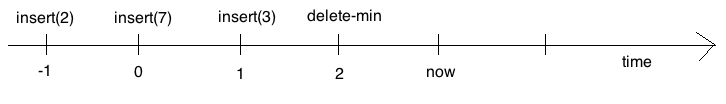
\includegraphics{timeline.png}}
\end{figure*}



Usually, operations are appended at the end of the time line (present time). With retroactive data structures we can do that in the past too.

\section{Retroactivity}

The following operations are supported by retroactive DS:

\begin{itemize}
\item {\em Insert(t, update)} - inserts operation ``update'' at time $t$
\item {\em Delete(t)} - deletes the operation at time $t$
\item {\em Query(t, query)} - queries the DS with a ``query'' at time $t$
\end{itemize}

Uppercase Insert indicates an operation on retroactive DS, lowercase update is the operation on the actual DS.

You can think of time $t$ as integers, but a better approach is to use an order-maintanance DS to avoid using non-integers (in case you want to insert an operation between times $t$ and $t+1$), as mentioned in the first lecture.

There are three types of retroactivity:
\begin{itemize}
\item {\em Partial} - Query always done at $t = \infty$ (now)
\item {\em Full} - Query at any time $t$ (possibly in the past)
\item {\em Nonoblivious} - Insert, Delete, Query at any time $t$, also if an operation modifies DS, we must say which future queries are changed.
\end{itemize}

\subsection{Easy case with commutativity and inversions}

Assume the following hold:
\begin{itemize}
\item {\em Commutative updates:} $x.y = y.x$ ($x$ followed by $y$ is the same as $y$ followed by $x$); that is the updates can be reordered $\Rightarrow$ Insert(t, op) = Insert(now, op).
\item {\em Invertible updates:} There exists an operation $x^{-1}$, such that $x.x^{-1} = \emptyset \Rightarrow$ Delete(t, op) = Insert(now, op$^{-1}$)
\end{itemize}

\subsubsection{Partial retroactivity}

These two assumptions allow us to solve some retroactive problems easily, such as:
\begin{itemize}
\item {\em hashing} 
\item {\em array} with operation $A[i] += \Delta$ (but no direct assignment)
\end{itemize}

\subsection{Full retroactivity}

First, lets define the {\bf search problem}: maintain set $S$ of objects, subject to insert, delete, query($x, S$).

{\bf Decomposable search problem} [1980, 2007]: same as the search problem, with a restriction that the query must satisfy:
query($x, A \cup B) = f($query$(x, A), $query($x, B))$, for some function $f$ computed in $O(1)$ (sets $A$ and $B$ may overlap). Examples of problems with such a function include:

\begin{itemize}
\item {\em Dynamic nearest neighbor}
\item {\em Successor on a line}
\item {\em Point location}
\end{itemize}

\begin{claim}
Full Retroactivity for decomposable search problems (with commutativity and inversions) can be done in $O(\lg{m})$ factor overhead both in time and space (where $m$ is the number of operations) using {\bf segment tree} [1980, Bentley and Saxe \cite{bs}]
\end{claim}

\begin{figure*}[ht]
  \centering
  \leavevmode
  \scalebox{.6}{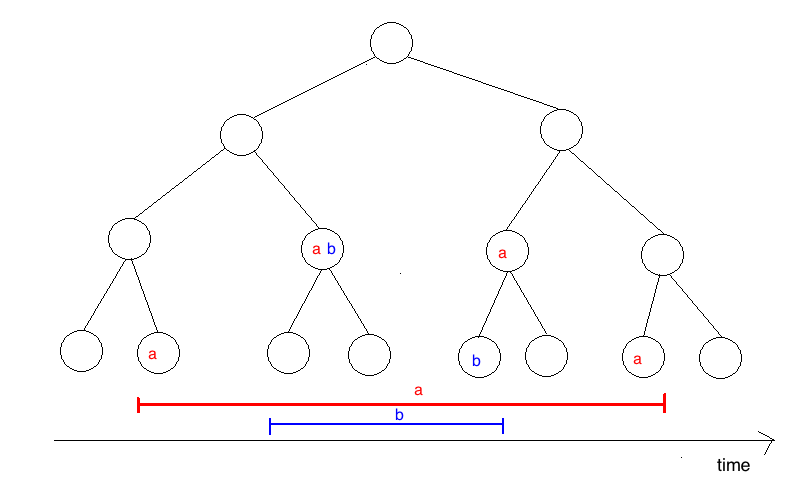
\includegraphics{segment_tree.png}}
  \caption{Segment Tree}
\end{figure*}

We want to build a balanced search tree on time (leaves represent time). Every element ``lives'' in the data structure on the interval of time, corresponding to its insertion and deletion. Each element appears in $\lg{n}$ nodes.

To query on this tree at time $t$, we want to know what operations have been done on this tree from the beginning of time to $t$. Because the query is decomposable, we can look at $\lg{n}$ different nodes and combine the results (using the function $f$). 

\subsection{General case of full retroactivity}

{\bf Roll back method}: 
\begin{itemize}
\item write down a (linear) chain of operations and queries
\item change $r$ time units in the past with factor $O(r)$ overhead. 
\end{itemize}

That's the best we can do in general. 

Lower bound: $\Omega (r)$ overhead necessary.

Proof: Data Structure maintains 2 values (registers): $X$ and $Y$, initially $\emptyset$. The following operations are supported: $X = x$, $Y += \Delta$, $Y = X.Y$, query '$Y?$'. Perform the following operations (Cramer's rule):
$$Y += a_n, X = X.Y, Y += a_{n-1}, X = X.Y, \ldots, Y += a_0$$


which is equivalent to computing $$Y = a_n X^{n} + a_{n-1} X^{n-1} + ... + a_0$$

Now, execute Insert($t = 0, X=x$), which changes where the polynomial is evaluated. This cannot be done faster than re-evaluating the polynomial. In history-independent algebraic decision tree, for any field, independent of pre-processing of the coefficients, need $\Omega(n)$ field operations (result from 2001), where $n$ is the degree of the polynomial.

\subsection{Cell-probe problem}

How many integers (words) of memory do you need to read to solve your problem? (gives a lower bound on running time).

Claim: $\Omega(\sqrt{\frac{r}{\lg{r}}})$.

{\bf OPEN} problem: $\Omega(r)$.

Proof of the lower bound claim:
\begin{itemize}
\item DS maintans $n$ words (integers of $w \ge \lg{n}$ bits). 
\item Arithmetic operations are allowed. 
\item Query = what is the value of an integer?
\item Compute FFT. 
\item Retroactively change the words $\Rightarrow$ Dynamic FFT. 
\item Changing $x_i$ requires $\Omega(\sqrt{n})$ cell probes.
\end{itemize}

\subsection{Priority Queues}
Now, let us move onto some more positive results.  Priority queues represent a DS where retroactive operations potentially create chain reactions but we have still obtained some nice results for.  The main operations are $insert$ and $delete$-$min$ which we would like to retroactively $Insert$ and $Delete$.

\begin{claim}
	It is possible to implement a partially retroactive priority queue with only $O(\lg n)$ overhead per partially retroactive operation.
\end{claim}

Because of the presence of $delete$-$min$, the set of operations on priority queues is non-commutative.  The order of updates now clearly matters, and $Insert$ing a $delete$-$min$ retroactively has the potential to cause a chain reaction which changes everything that comes afterward. Partially retroactive priority queues are described in a paper by Demaine, Iacono, and Langerman \cite{dil}. \\

To develop an intuition for how our DS changes given a retroactive operation, it is helpful to plot it on a two dimensional plane.  The $x$-axis represents time and $y$-axis represents key value. Every $insert(t,k)$ operation creates a horizontal ray that starts at point $(t,k)$ and shoots to the right (See Fig. \ref{fig-pqinsert}).

\begin{figure}[ht]
	\rule{\textwidth}{0.005in}
  \begin{center}
    \scalebox{.8}{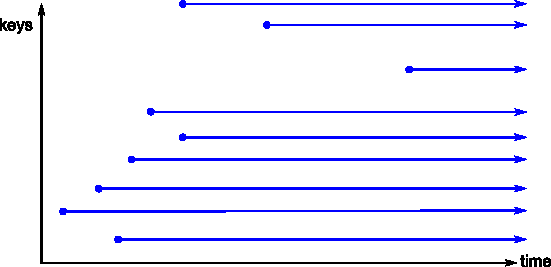
\includegraphics[width=6in]{pqinsert.pdf}}
  \end{center}

  \caption{\small Graph of priority queue featuring only a set of $insert$s}
  \label{fig-pqinsert}
	\rule{\textwidth}{0.005in}
\end{figure}

Every $delete$-$min()$ operation creates a vertical ray that starts at $(t,-\infty)$ and shoots upwards, stopping at the horizontal ray of the element it deletes. Thus, the horizontal ray becomes a line segment with end points $(t,k)$ and $(t_k,k)$, where $t_k$ is the time of key $k$'s deletion.

This combinations of inserts and deletes creates a graph of nonintersecting upside down ``L'' shapes, where each L corresponds to an $insert$ and the $delete$-$min()$ that deletes it.  Elements which are never deleted remain rightward rays. Figure \ref{fig-pqdel} demonstrates this by adding a few $delete$-$min$s to our previous graph of only $insert$s.

\begin{figure}[ht]
	\rule{\textwidth}{0.005in}
  \begin{center}
    \scalebox{.8}{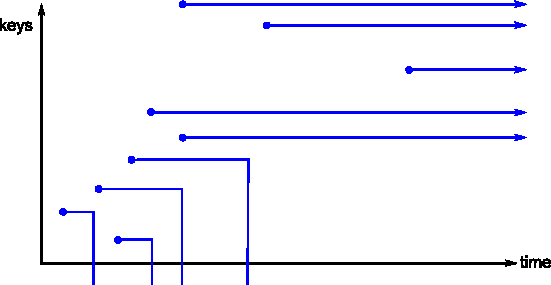
\includegraphics[width=6in]{pqdel}}
  \end{center}

  \caption{\small Adding $del$-$min()$ operations leads to these upside down ``L'' shapes.}
  \label{fig-pqdel}
	\rule{\textwidth}{0.005in}
\end{figure}

The rest of the discussion will focus on $Insert(t,$``$insert(k)$''$)$.  It should be easy enough to convince yourself that $Delete(t,$``$delete$-$min$''$)$ has equivalent analysis if you think about Delete as inserting the deleted element at the time of deletion. 

\begin{figure}[ht]
	\rule{\textwidth}{0.005in}
  \begin{center}
    \scalebox{.8}{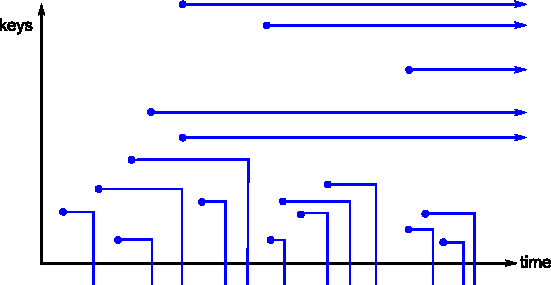
\includegraphics[width=6in]{pqlview}}
  \end{center}

  \caption{\small An L view representation of a priority queue with a more complicated set of updates}
  \label{fig-pqlview}
	\rule{\textwidth}{0.005in}
\end{figure}

Consider the priority queue represented by figure \ref{fig-pqlview}.  It's similar to the previous ones seen but with more inserts and deletes to better illustrate the chain-reactions of retroactive operations.  Figure \ref{fig-pqretro} shows what happens when elements are retroactively inserted.  The retroactive operations and their chain reactions are shown in red.  The cascading changes add up fast.

\begin{figure}[ht]
	\rule{\textwidth}{0.005in}
  \begin{center}
    \scalebox{.8}{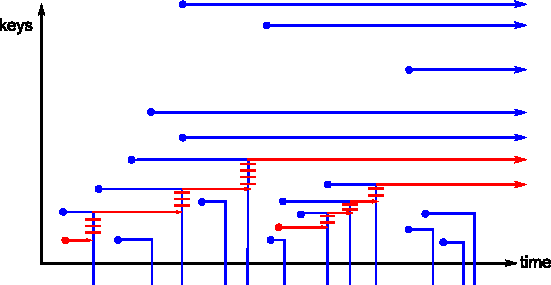
\includegraphics[width=6in]{pqretro}}
  \end{center}

  \caption{\small Retroactive inserts start at red dots and cause subsequent $delete$-$min$ operations to effect different elements as shown.}
  \label{fig-pqretro}
	\rule{\textwidth}{0.005in}
\end{figure}

However, since we're only requiring partial retroactivity we only need to determine what element $Insert(t,$``$insert(k)$''$)$ inserts into $Q_{now}$ where $Q_{now}$ is the priority queue at the present time.  Naively, it is easy to see that the element inserted at $Q_{now}$ is: $\max\left\{k,k' \mid k' \text{ deleted at time} \ge t\right\}$.  That is, the element that makes it to the ``end'' is the biggest element that was previously deleted (ie. the end of the chain-reaction shown in Figure 3) or simply $k$ if it is bigger than those (ie. the insert caused no chain reactions).

\paragraph{Problem:} Maintaining ``deleted'' elements is hard.  It requires us to maintain the various chain-reactions which isn't efficient.  Instead, we would like to simply keep track of inserts.  Such a transformation is possible as long as we define the new concept of ``bridges''.

\begin{definition}
	We define time $t$ to be a bridge if $Q_t \subseteq Q_{now}$.
\end{definition}

This simply means that all of the elements present at a bridge $t'$ are also present at $t_{now}$.  You can think of bridges as separating the chaotic chain-reactions that happen during retroactive operations as seen in figure \ref{fig-pqbridge}.

If $t'$ is the bridge preceding time $t$, then \\ $\max \left\{ k' \mid k' \text{ deleted at time} \ge t \right\} = \max \left\{ k' \notin Q_{now} \mid k' \text{ inserted at time} \ge t' \right\}$


\begin{figure}[ht]
	\rule{\textwidth}{0.005in}
  \begin{center}
    \scalebox{.8}{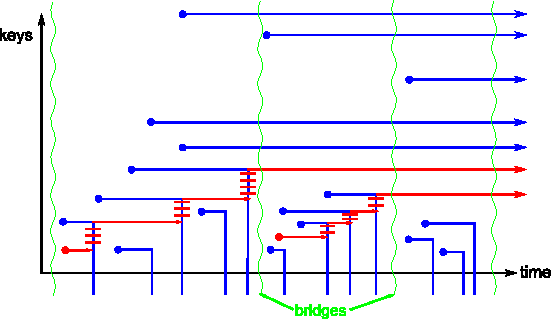
\includegraphics[width=6in]{pqbridge}}
  \end{center}

  \caption{\small Bridges have been inserted as green wavy lines. Notice how they only cross elements present to the end of visible time.}
  \label{fig-pqbridge}
	\rule{\textwidth}{0.005in}
\end{figure}

With that transformation, we only need to maintain three data structures which will allow us to perform partially retroactive operations with only $O(\lg n)$ overhead.

\begin{itemize}
\item We will store $Q_{now}$ as a balanced BST.  It will be changed once per update.
\item We will store a balanced BST where the leaves equal insertions, ordered by time, and augmented with $\forall \text{ node } x: \max\left\{ k' \notin Q_{now} \mid k' \text{ inserted in } x \text{'s subtree} \right\}$.

\item Finally, we will store a balanced BST where the leaves store all updates, ordered by time, and augmented by the following: \\

\[
\left\{ \begin{array}{ll}
$0$ & \mbox{for inserts with $k \in Q_{now}$} \\
$+1$ & \mbox{for other inserts, $k \notin Q_{now}$} \\
$-1$ & \mbox{for $delete$-$min$s} \\
\end{array}
\right. \\
\]

as well as subtree sums.

\end{itemize}

Now, we have to uses these data structures to execute our $Insert$.  This can be done in $O(\lg n)$ with the following steps.

\begin{itemize}
	\item First, for an $Insert$ at time $t$ we must find the preceding bridge at time $t'$.  Using our BBST of all updates, we know that a bridge is a time(leaf) at which has a prefix of updates summing to 0 (with respect to the augmentation). This is possible in $O(\lg n)$ time due to the stored subtree sums.  In brief, traverse the tree to find $t$, calculating the prefix sum as you descend.  If $t$ has a prefix sum of $0$ then we're done. Otherwise, walk back up the tree to find the preceding update with a prefix sum of $0$.

\item Next, in our BBST of insertions we descend to $t'$ and work back up the tree looking for the maximum node not already in $Q_{now}$.  Because of the augmentation we store, this can be done in $O(\lg n)$ time.

\item Finally, there are a collection of steps related to updating the data structures once we make our update, but given our data structures it should be easy to convince yourself that it can be done in $O(\lg n)$ time.
\end{itemize}

\subsection{Other Structures}
\begin{itemize}
\item{\emph{queue:}} $O(1)$ partial, $O(\lg m)$ full
\item{\emph{deque:}} $O(\lg m)$ full
\item{\emph{union-find (incremental connectivity):}} $O(\lg m)$ full
\item{\emph{priority-queue:}} $O(\sqrt{m}\lg m)$ full. This comes from the fact that any partially retroactive DS can be made fully retroactive with a $O(\sqrt{m})$ factor overhead.  It's an {\bf OPEN} problem whether or not we can do better.
\item{\emph{successor:}} This was actually the motivating problem for retroactivity.  $O(\lg m)$ partial because it's a search problem. $O(\lg^2 m)$ full because it's also decomposable.  However, Giora and Kaplan gave us a better solution of $O(\lg m)$ \cite{gk}!  This new algorithm uses many data structures we'll learn about later; including fractional cascading (L3) and vam Emde Boas (L11).

\end{itemize}

\subsection{Nonoblivious Retroactivity}

Nonoblivious retroactivity was introduced in a paper by Acar, Blelloch, and Tangwongsan to answer the question, ``What about my queries? \cite{abt}''  Usually, when we use a data structure algorithmically (e.g. priority queue in Dijkstra) the updates we perform depend on the results of the queries.

To solve this problem we can simply add queries to our time line (fig. \ref{fig-nrtl}).

\begin{figure}[ht]
	\rule{\textwidth}{0.005in}
  \begin{center}
    \scalebox{.5}{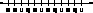
\includegraphics[width=6in]{nrtl}}
  \end{center}

  \caption{\small Time line of updates \emph{and} queries.}
  \label{fig-nrtl}
	\rule{\textwidth}{0.005in}
\end{figure}

The notion of dependence depends upon the user, but we still want to do something reasonable.  Now, when we make a retroactive update, we want our DS to tell us the location of the first query which changed as a result (e.g. the first error).  Then we only have to re-run the algorithm from that first erroneous query.  Our assumption is that the algorithm does this by $Delete$ing each wrong update and re-$Insert$ing the proper update in a strict left to right order such that each update is lower on the time-line than all errors.

After fixing each error, we can go back to using our retroactive DS in the usual way with no restrictions.

\paragraph{Priority-Queues:} Our priority queues will support insert, delete, and min in $O(\lg m$ time per operation.

Because we have retroactive queries now, we separate the query and updates into different operations.  Our matching retroactive queries will be Insert, Deleate, and Min.  We will visualize our data structure using a similar 2D plane as before as seen in figure \ref{fig-nrpq}.

\begin{figure}[ht]
	\rule{\textwidth}{0.005in}
  \begin{center}
    \scalebox{.8}{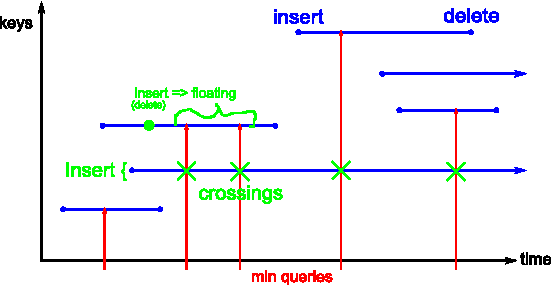
\includegraphics[width=6in]{nrpq}}
  \end{center}

  \caption{\small 2D representation of DS.  $Insert$ing an $insert$ leads to crossings as shown.  $Insert$ing a $delete$ leads to floating errors as shown.}
  \label{fig-nrpq}
	\rule{\textwidth}{0.005in}
\end{figure}

If we Insert an insert as shown in fig \ref{fig-nrpq} then we get errors at each crossing.  In our DS we will keep the `incorrect' picture, but keep track of the errors.  We will tell the algorithm where the first error (crossing) is and it will potentially Delete the query and re-Insert the operation thus getting the correct result.

However, we don't jump to the next error after this is done. Our assumption is that the algorithm will, based on the new query, do various updates which may even delete the new element before any further crossings.

Deleting a deletion is similar to Inserting an insertion as they both cause crossing errors.

The other two cases are Deleting an insertion and Inserting a deletion which cause floating errors.  These are situations where queries return `floating' values because they refer to a segment which is no longer there.

Both crossing and floating errors can be seen in figure \ref{fig-nrpq}.

We maintain the following two details

\begin{itemize}
\item First, we maintain the lowest leftmost crossing. This is equivalent to the leftmost lowest crossing. This is because of the invariant that all crossings involve horizontal segments with left endpoint left of \emph{all} errors.
\item Next, we maintain the left most floating error on each row separately.
\end{itemize}

\paragraph{Example:} $Insert(t, \text{``min''})$.  When adding a new query what is the first ray that I hit.  This only involves the horizontal segments which are being inserted and deleting.  This problem is called \emph{upward ray shooting among dynamic segments}.  We can solve it in $O(\lg m)$ per operation.  This turns out to be the same as the fully retroactive successor problem mentioned earlier which was proved to be $O(\lg m)$ in \cite{gk}.

The other cases are similar but you also need to use rightward ray shooting.

%\bibliography{mybib}
\bibliographystyle{alpha}

\begin{thebibliography}{77}

\bibitem{dil}
Erik D. Demaine, John Iacono, Stefan Langerman: \emph{Retroactive data structures}. SODA 2004: 281-290

\bibitem{dil2}
Erik D. Demaine, John Iacono, Stefan Langerman: \emph{Retroactive data structures}. ACM Transactions on Algorithms 3(2): (2007)

\bibitem{gk}
Yoav Giora, Haim Kaplan: \emph{Optimal dynamic vertical ray shooting in rectilinear planar subdivisions} ACM Transactions on Algorithms 5(3) (2009)

\bibitem{abt} Umut A. Acar, Guy E. Blelloch, Kanat Tangwongsan: \emph{Kinetic 3D convex hulls via self-adjusting computation}. Symposium on Computational Geometry 2007: 129-130

\bibitem{fhm}
Gudmund Skovbjerg Frandsen, Gudmund Skovbjerg Frandsen, Peter Bro Miltersen: \emph{Lower Bounds for Dynamic Algebraic Problems}. Information and Computation 171(2): 333-349 (2001)

\bibitem{bs}
Jon Louis Bentley, James B. Saxe: \emph{Decomposable Searching Problems I: Static-to-Dynamic Transformation}. J. Algorithms 1(4): 301-358 (1980)

\end{thebibliography}

\end{document}
